%!TEX root = ../thesis.tex

\section{背景}
近年, 配膳ロボットや警備案内ロボットなどの需要が高まり, 自律的に移動できることが求められている. これらのロボットはLiDAR, ホイールオドメトリ, IMUなどの様々なセンサから得られるデータに基づいて作成された占有格子地図を用いてナビゲーションを行う. \par また, 本研究グループでは, end-to-end学習により, 視覚に基づく経路追従行動をオンラインで模倣する手法を提案し, その有効性を実験により検証してきた. 岡田らが提案した手法では\figref{Fig:old}に示すようなLiDARやホイールオドメトリなどを入力として生成したナビゲーションの行動を, カメラ画像を入力とする行動に模倣する\cite{okada-si2020}\cite{okada-si2021}. これにより, 地図を用いたナビゲーションと視覚に基づく経路追従行動の2つのナビゲーション手段が得られるため, 状況に応じて高い信頼性が見込まれる方を選択することで, 経路追従を継続できる可能性が高まる. 

% \newpage
% 岡田らは\figref{Fig:tsudanuma2-3}のように地図ベースのナビゲーションによる出力を模倣することで, 経路追従行動を獲得した\cite{okada-si2020}. \figref{Fig:okada-si2020}に示すような, LiDAR, オドメトリを入力としたナビゲーションの出力をend-to-endで模倣学習し, 学習後はカメラ画像を入力とした学習器の出力により, 一定の経路において周回が可能であることが確認された. 

\newpage
\begin{figure}[h]
     \centering
     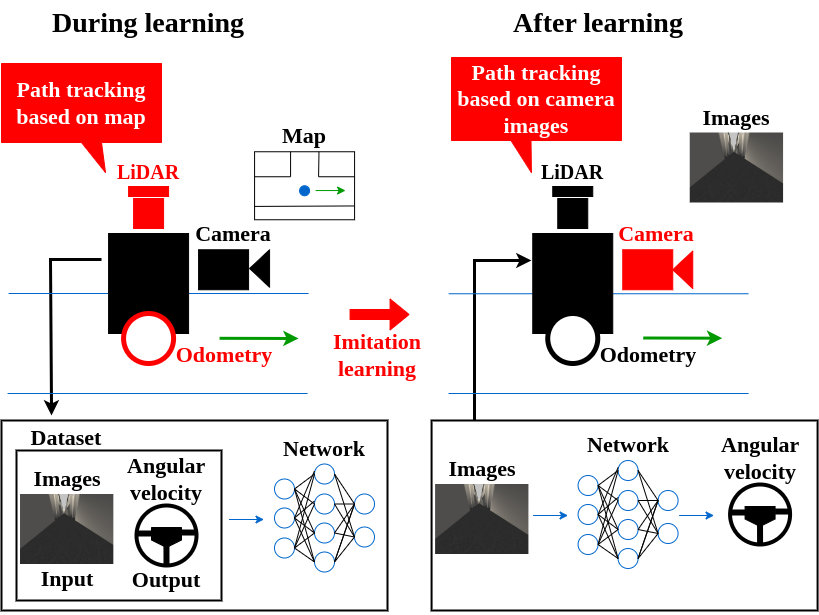
\includegraphics[keepaspectratio, scale=0.3]
     {images/old.png}
     \caption{Path-tracking by end-to-end imitation learning}
     \label{Fig:old}
     \end{figure}

\section{関連研究}
視覚を入力として, end-to-end学習により経路追従を模倣する手法をいくつか紹介する. 例えば, Bojarskiらは人が操作したステアリングの角度をend-to-end学習することで経路追従する手法を提案した. \figref{Fig:bojaski}に示すように学習器に, 3つのカメラ(左・中央・右)の画像と対応するステアリングの角度を入力する. 学習後は出力されたステアリングの角度のみで自律走行することが確認された\cite{bojaski}. 

\begin{figure}[h]
     \centering
     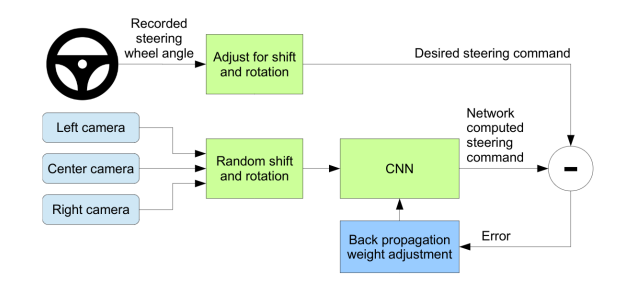
\includegraphics[keepaspectratio, scale=0.45]
     {images/bojaski.png}
     \caption{Training the neural network(source: \cite{bojaski})}
     \label{Fig:bojaski}
     \end{figure}

また, Jing Biらは, 歩行者の多い環境における経路追従行動の模倣に取り組んだ. 具体的には, \figref{Fig:jing-bi}に示すようなフレームワークを用いて, \figref{Fig:pedestrian}のような歩行者のいる状況に合わせて, 人が操作しながらデータ収集を行う. ステージ1では「どの状況にいるのか」を判断する. ステージ2では分類結果に基づいて「具体的にどう動くか」を決定する. 経路から外れたり, 人と衝突したりなどのエラーに遭遇しそうな場合には人が介入を行う. そして, 介入の前後を含めてポリシーを更新する. これにより, 歩行者がいる場合でも経路追従できることが確認された\cite{Jing}. 

\begin{figure}[h]
     \centering
     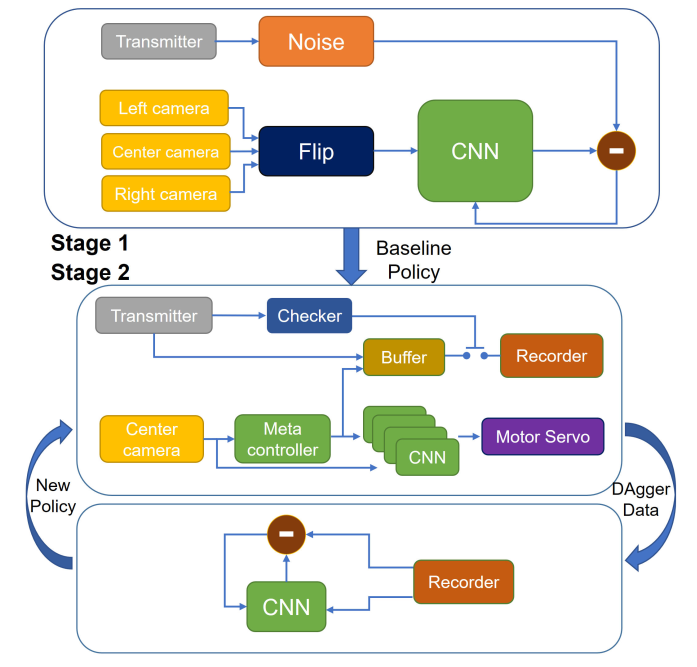
\includegraphics[keepaspectratio, scale=0.4]
     {images/jing-bi.png}
     \caption{Framework overview(source: \cite{Jing})}
     \label{Fig:jing-bi}
     \end{figure}

\begin{figure}[h]
     \centering
     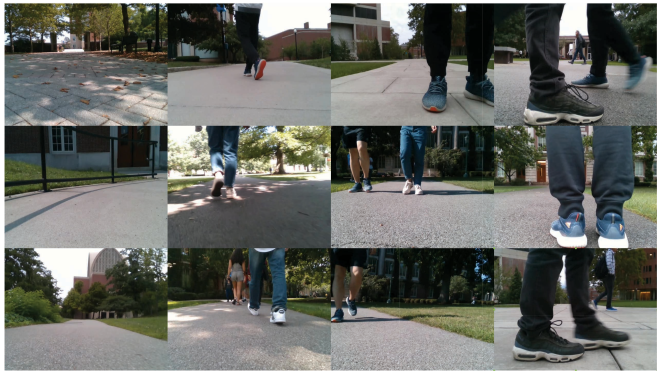
\includegraphics[keepaspectratio, scale=0.4]
     {images/pedestrian.png}
     \caption{Robot navigation in a pedestrian environment(source: \cite{Jing})}
     \label{Fig:pedestrian}
     \end{figure}

% \vspace{20mm}
\newpage
これらの手法が人の手動操作を模倣しているのに対して, 岡田らの手法は自動運転を模倣する点が異なる. しかし, 岡田らの手法では, データ収集及び学習を行うために, ロボットを経路に沿って走行させ続けることが必要である. そのため, 経路追従の成功率を上げるためにロボットを長時間走行させ続ける必要があり, それが問題となっていた. 

\newpage
\section{目的}
本論文では, 岡田らの手法で問題となっていた学習に要する時間を短縮するために, 事前に収集した画像と行動を用いて, 経路追従行動をオフラインで学習する手法(以後, オフライン手法と呼ぶ)を提案する. これにより, 岡田らの手法で問題となっていた学習時間の短縮を目的とする. なお, オフラインで模倣学習することは, 他の研究でも行われていることであるが, そのデータセットを自動で収集する点が本手法の特徴である. また, 実ロボットにオフライン手法を適用することを念頭において, 経路周辺の視覚情報がどれだけ必要であるかを, シミュレータを用いた実験により明らかにすることも目的とする.
\section{論文構成}
本論文の構成は以下に述べる通りである. 第1章では, 研究を行う背景や目的を述べた. 第2章では, 研究に関連する要素技術, 第3章では, 従来手法について説明する. 第4章では, 提案手法について説明し, 第5章と第6章では, 実験について説明する. そして, 第7章では, 本研究の結論を述べる. 
     
